% !TEX root = main.tex
\documentclass[11pt]{article}
\usepackage[preprint]{acl}
\usepackage{times}
\usepackage{latexsym}
\usepackage[T1]{fontenc}
\usepackage[utf8]{inputenc}
\usepackage{booktabs}
\usepackage{microtype}
\usepackage{graphicx}
\usepackage{amsmath}

\newcommand{\cps}{\textsc{cps}}
\title{Are Auxiliary Cues Uniquely Informative for Coarse Verb-Class\\Learning in Masked Language Models Trained on CHILDES?}
\author{Yiyang Liu \\ 
  Shanghai Jiao Tong University \\
  \href{mailto:brayden615@sjtu.edu.cn}{brayden615@sjtu.edu.cn}}

\begin{document}
\maketitle

\begin{abstract}
Can English auxiliaries support coarse expectations about the class of a novel verb beyond the lexical contexts in which they occur? We train small masked language models from scratch on child-directed speech and evaluate them using leakage-controlled baselines, matched corpus-damage controls, an AUX-identity-shuffle intervention, and nonce forms embedded in held-out local templates. Verb-class accuracy rises from 53.7\% to 72.2\% as the amount of training data increases. An AUX-only baseline achieves 30.5\% accuracy, compared with 44.5\% for POS frames and 52.0\% for lexical context. In a five-seed natural-corpus experiment, replacing AUX identities with a shared token reduces class preference by 0.144 relative to unmodified input, but the reduction is not reliably greater than that produced by either matched-damage control. In the nonce-form experiment, shuffling AUX identities reduces cross-template accuracy by 3.27 percentage points and class preference by 0.096; matched-function ablation also reduces class preference. These results indicate that auxiliary information contributes one cue within a redundant distributional system, but they cannot distinguish between the absence of an AUX-specific effect and an effect too small for the present design to detect.
\end{abstract}

\section{Introduction}

Learning a verb requires identifying the event or relation it denotes and determining how the language lexicalizes that concept. Syntactic bootstrapping proposes that a verb's distribution over sentence structures constrains its possible meanings \citep{gleitman1990,fisher1991}. Children map novel verbs to different event interpretations when the verbs occur in different argument-structure frames \citep{naigles1990,fisher2010}. These findings show that structure guides interpretation, but leave open which observable cues make it accessible and how learners combine them.

Function words provide one possible entry point: they are frequent, occupy stable structural positions, and often align with phrase boundaries \citep{decarvalho2019,yang2026}. Infants can also distinguish lexical words from grammatical words on the basis of their perceptual correlates \citep{shi1999}, although the present text-only models do not receive those phonological cues. English auxiliaries mark tense, aspect, modality, negation, and clause type; the environments in which they occur may therefore correlate with broad verb classes. However, auxiliaries also covary with lexical content, local frames, and other closed-class material. Removing them changes both the cue of interest and the input distribution. An ablation effect alone therefore cannot separate auxiliary information from corpus damage.

We address three questions. Can small masked language models learn coarse verb-class expectations from child-directed text? Does replacing auxiliary identities impair learning more than matched forms of corpus damage? Do stable auxiliary--context mappings support transfer to unseen verb forms in held-out local templates?

We use matched-damage controls, identity shuffling, and nonce forms in held-out templates to separate total cue contribution from cue specificity and test transfer beyond familiar verb identities and exact local frames. We compare auxiliary information with leakage-controlled lexical and structural baselines across training scales; across these analyses, auxiliary patterns are informative, but not uniquely so.

For the intervention comparisons, matched-damage controls preserve the overall scale and distribution of corpus changes, while identity shuffling preserves the auxiliary unigram distribution. The nonce analysis then evaluates whether an exposure manipulation affects held-out templates rather than only familiar verb identities. These contrasts are designed to test the evidence available to the model, not to identify a causal mechanism in child learning.
\section{Background and related work}

\subsection{From structural frames to observable cues}

Subcategorization frames provide probabilistic evidence about semantic properties such as participant number and event type \citep{gleitman1990,fisher1991}. The proposal concerns distributions across frames, not a deterministic mapping from a single surface pattern to a meaning. Behavioral evidence reflects this distinction: two-year-olds use transitive and intransitive frames to interpret novel actions \citep{naigles1990}, while later work places these effects within a system that also integrates referential and lexical evidence \citep{fisher2010}.

Identifying these frames poses a further problem because learners must locate structure before knowing all content words. Function words and prosody can constrain the syntactic category of a novel word: 18-month-olds use these cues together to distinguish object-denoting from action-denoting interpretations \citep{decarvalho2019}. Distributional analyses of child-directed speech likewise show that surrounding-word contexts and frequent frames can support the induction of grammatical categories, including nouns and verbs \citep{mintz2002,mintz2003}. More broadly, function words are frequent, reliably associated with syntactic contexts, and aligned with boundaries across languages; preserving these properties improves structural learning in neural models \citep{yang2026}. Multiple-cue accounts of verb learning emphasize that such distributional information can complement other language-internal cues \citep{christiansenmonaghan2006}. These studies concern category and structure learning rather than semantic distinctions \emph{within} the verb category. We test the latter.

\subsection{Language models as controlled learners}

CHILDES provides naturalistic transcripts of child--caregiver interaction \citep{macwhinney2000}, and BabyLM provides a reproducible setting for sample-efficient pretraining on developmentally motivated text \citep{warstadt2023}. Compact RoBERTa-style models trained on child-directed input can acquire non-trivial grammatical generalizations at this scale \citep{huebner2021}. Computational acquisition accounts have also jointly learned syntax and lexical semantics when supplied sentence-level meaning representations \citep{abend2017}; our models receive text only. Controlled comparisons indicate that local discourse properties of child-directed speech can matter, but do not demonstrate a general advantage over other training distributions \citep{feng2024}. Neural models and children also differ in their sensitivity to frequency, concreteness, and lexical class \citep{chang2022}. We therefore treat masked LMs as controlled distributional learners rather than cognitive models of children.

Corpus intervention can test whether a distributional regularity is useful to a model when architecture and evaluation are held fixed. It cannot establish that children use the same mechanism. A model-level claim of cue specificity also requires controls that produce comparable amounts and locations of corpus damage. Building on evidence that function-word statistics support structural learning \citep{yang2026}, we ask whether auxiliary identity supports verb-class learning beyond correlated lexical, frame, and function-word cues.

\section{Data and task}

\paragraph{Corpus.}
We use the CHILDES component distributed with the BabyLM 2026 Strict release, with source identity verified by SHA-256. The cleaned corpus contains 904,228 utterances and 6.953M whitespace-delimited tokens. POS annotation and punctuation segmentation yield 904,222 model records and 8.449M token units; the fixed 80/10/10 record-level split places 723,377 records and 6.760M units in training. We retain only parental speech directed to children and lowercase the utterances. We obtain coarse tags with spaCy 3.4.4 and the \emph{en\_core\_web\_sm} 3.4.1 model, using the Universal POS inventory \citep{demarneffe2021}; the tags are used only to construct interventions, baselines, and local-frame analyses, never as model-input tokens. All conditions share a 4,000-type byte-level BPE tokenizer, a BPE-based subword scheme \citep{sennrich2016}, trained on the unmodified training split. We report both token counts because annotation and punctuation segmentation change the counting unit.

\paragraph{Verb classes.}
The researcher-defined evaluation ontology contains five coarse classes: transitive action, intransitive, ditransitive transfer, mental/communication, and perception. The first three partly encode argument-structure distinctions, whereas the latter two are broader lexical-semantic classes; the ontology therefore does not isolate semantics from valency. The 600 evaluation items are balanced at 120 per class and come from 600 distinct corpus records, with 76 target surfaces from 39 lemmas. The class-balanced candidate set contains 21 surfaces per class. At evaluation, only the target verb position is masked; all remaining lexical context is visible. The task thus measures distributional compatibility with this mixed, coarse class ontology, not recovery of a complete lexical meaning.

\paragraph{Metrics.}
The preregistered primary metric is the class preference score
\begin{equation}
\begin{aligned}
  \cps(x,y)={}&\operatorname{mean}_{v\in y}\log p(v\mid x) \\
  &-\operatorname{mean}_{v\notin y}\log p(v\mid x),
\end{aligned}
\end{equation}
where $y$ is the target class and $v$ ranges over the candidate surfaces. The secondary verb-class accuracy metric selects the highest-scoring candidate surface and assigns its verb class as the prediction. Scores for multi-piece candidates use length-normalized subword log probabilities.

\paragraph{Annotation audit.}
The exhaustive lexical audit classifies 935,294 of 935,364 AUX-tagged events as instances of canonical or otherwise accepted auxiliary forms; 70 are flagged as likely mistags or transcription/tokenization artifacts. For a deterministic sample of 500 contexts, the automatic labels are withheld from the independent annotator. The reported count is therefore a lexical audit, not human-validated tagging accuracy.

\section{Model and interventions}

All main models are two-layer RoBERTa-style masked LMs with 946,208 trainable parameters, a hidden size of 128, four attention heads, an intermediate size of 512, and dropout of 0.1. They use bidirectional masked-token prediction \citep{devlin2019} and train for five epochs with a batch size of 16, a learning rate of $5\times10^{-4}$, weight decay of 0.01, and a masking probability of 0.15. Hyperparameters are fixed before the confirmatory natural-corpus experiment; its test results are not used for tuning. We train five independently initialized models per condition.

The five natural-corpus conditions are:
\begin{enumerate}
  \item \textbf{Original}: unchanged training input.
  \item \textbf{AUX-identity ablation}: all 748,105 training AUX events are replaced by a dedicated ablation token. This removes form identity while retaining the occurrence and position of an AUX event.
  \item \textbf{Matched-content ablation}: an equal number of content-word positions are ablated, prioritizing positions in the same utterance. This maximizes overlap in affected utterances but cannot match AUX position and frequency.
  \item \textbf{Matched-function ablation}: non-AUX closed-class positions are selected to match token frequency, relative utterance position, and distance to the nearest verb.
  \item \textbf{AUX-identity shuffle}: the AUX unigram multiset is preserved while form--context mappings are deterministically deranged.
\end{enumerate}
All interventions apply only to training. Development and test hashes are identical across conditions.

\section{Experiments}

\subsection{Scale and leakage-controlled baselines}

We compare performance at 720k tokens, 2M tokens, and the full training scale under the same five-epoch schedule; training scale therefore also changes the number of optimization updates. Leakage-controlled baselines never observe the target token: a class-frequency baseline, AUX-only Naive Bayes, exact local POS-frame counts, and lexical-context Naive Bayes. Five untrained initializations quantify architecture and tokenizer bias. These comparisons ask how much signal auxiliaries contain and how it compares with other observable context, not whether AUX adds predictive value conditional on all other cues.

\begin{figure*}[tb]
  \centering
  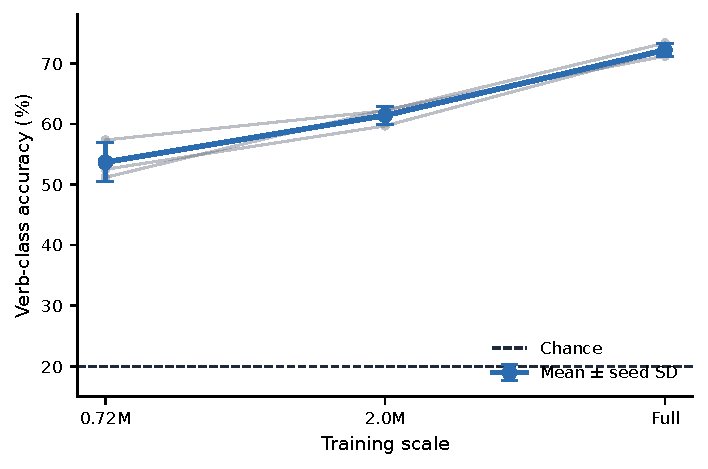
\includegraphics[width=.48\linewidth]{figures/learning_curve.pdf}\hfill
  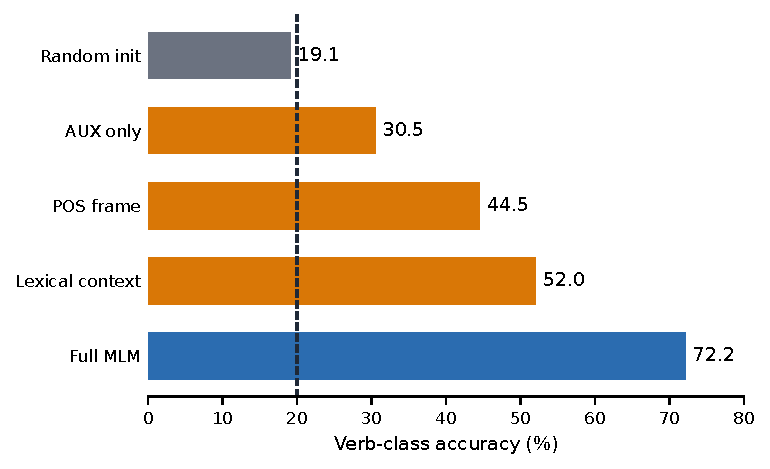
\includegraphics[width=.48\linewidth]{figures/baseline_gradient.pdf}
  \caption{Verb-class accuracy by training scale (left) and information source at full scale (right). The scale curve uses the three Original-condition checkpoints with seeds 2026--2028, which are also included in Table~\ref{tab:confirmatory}; Table~\ref{tab:confirmatory} adds seeds 2029--2030. Points are individual seeds; error bars show seed-level standard deviations. All statistical baselines exclude the target verb. The dashed line marks the 20\% balanced-class chance level.}
  \label{fig:scale-baselines}
\end{figure*}

\subsection{Corpus-level cue mechanism}

For every AUX form, we estimate class-conditional frequency, entropy, reliability, and mutual-information contribution in the training split. Each evaluation item receives a training-corpus AUX log-odds score for its target class. We correlate this score with accuracy and \cps{} separately by model seed. This analysis is diagnostic rather than causal because the item contexts contain other correlated cues.

\subsection{Nonce verbs across held-out templates}

Each class is assigned one corpus-absent nonce form that tokenizes into exactly two BPE pieces. We select 80 exposure items per class, all containing an auxiliary, and evaluate on 100 items per class whose exact local $\pm2$ POS frame does not occur in exposure. Starting from each of three full-corpus Original-condition checkpoints, we adapt on target-masked nonce exposures under four conditions: intact exposure, AUX-identity ablation, AUX-identity shuffle, and matched-function ablation. Adaptation uses eight epochs and a learning rate of $5\times10^{-5}$; evaluation contexts are always intact. The fixed nonce-to-class mapping makes within-mapping intervention contrasts paired, but it does not counterbalance nonce identity across classes.

\subsection{Confirmatory natural-corpus ablation}

The preregistered primary contrasts compare AUX-identity ablation with each matched control on \cps{}. An AUX-specific claim requires both hierarchical confidence intervals to exclude zero in the predicted direction and requires the predicted direction to be observed in at least four of the five seeds. We draw 10,000 paired hierarchical-bootstrap samples: each draw resamples model seeds, then resamples the 600 paired item differences within each selected seed \citep{efron1979}. This procedure does not separately resample verb, template, transcript, or child clusters. For the nonce contrasts, we report two-sided bootstrap $p$-values adjusted within the prespecified metric-by-intervention family using Holm's procedure \citep{holm1979}. We interpret intervals, adjusted tests, and seedwise directions jointly, following recommendations to make uncertainty reporting explicit in NLP experiments \citep{dror2018}.

\section{Results}

\subsection{Scale and available cue information}

Class accuracy increases from 53.7\% at 720k tokens to 61.4\% at 2M and 72.2\% at full scale (Figure~\ref{fig:scale-baselines}, left), a total gain of 18.5 points with no reversal across the three seeds. This is a fixed-epoch training-scale result, so it jointly reflects more text and more update steps. The 72.2\% full-scale value is the mean of seeds 2026--2028; the five-seed mean for the Original condition in Table~\ref{tab:confirmatory} is 71.1\% after adding seeds 2029--2030. AUX-only Naive Bayes reaches 30.5\%, 10.5 points above the 20\% balanced-class chance level but below exact POS frames (44.5\%), lexical context (52.0\%), and the trained model (72.2\%; Figure~\ref{fig:scale-baselines}, right). Thus, auxiliary statistics contain class information but explain substantially less than richer structural and lexical context.

\subsection{Corpus statistics and model behavior}

Across the three full-corpus seeds, AUX log-odds scores correlate with binary item-level accuracy ($r_{pb}=.20$--$.24$, all $p<.001$) and with \cps{} (Spearman $\rho=.15$--$.19$, all $p<.001$). Figure~\ref{fig:cue-behavior} shows closely aligned seed trajectories: mean preference is highest in the most positive AUX-log-odds decile, but the intermediate deciles are visibly non-monotonic. Thus, highly class-diagnostic auxiliary contexts coincide with stronger class preference, while AUX log-odds scores do not follow a simple dose--response ordering over all items. The associations remain modest and observational: they show that model success tracks auxiliary diagnosticity on average, not that auxiliaries alone cause successful predictions.

\begin{figure}[tb]
  \centering
  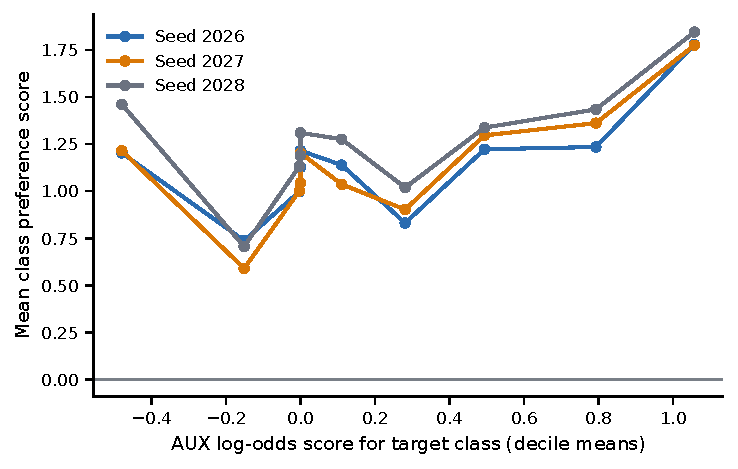
\includegraphics[width=.94\columnwidth]{figures/cue_behavior.pdf}
  \caption{Mean class preference by decile of the training-corpus AUX log-odds score for the target class. Each equal-count bin contains 60 evaluation items. Lines show three independently initialized full-corpus models; the plot is descriptive and does not establish a monotonic or causal relation.}
  \label{fig:cue-behavior}
\end{figure}

\subsection{Natural-corpus intervention}

Table~\ref{tab:confirmatory} reports both the secondary accuracy metric and the preregistered \cps{} metric for every training intervention.
\begin{table}[t]
\centering
\small
\setlength{\tabcolsep}{3pt}
\begin{tabular}{lrr}
\toprule
Training condition & Accuracy (\%) & \cps{} \\
\midrule
Original & 71.1 (1.8) & $1.169$ (0.061) \\
AUX-identity ablation & 61.0 (1.3) & $1.025$ (0.032) \\
Matched-content ablation & 68.5 (2.0) & $1.048$ (0.097) \\
Matched-function ablation & 69.1 (1.2) & $1.071$ (0.045) \\
AUX-identity shuffle & 60.8 (1.8) & $1.032$ (0.017) \\
\bottomrule
\end{tabular}
\caption{Natural-corpus results over five initialization seeds and the same 600 class-balanced items per seed. Parentheses give seed-level standard deviations; paired bootstrap contrasts are reported in the text.}
\label{tab:confirmatory}
\end{table}

Across five seeds, the Original condition obtains a mean \cps{} of 1.169, compared with 1.025 after AUX-identity ablation ($\Delta=-0.144$, 95\% CI [-0.207, -0.085], $p<.0001$). Relative to the matched-content control, the ablation difference is $\Delta=-0.023$ (95\% CI [-0.083, 0.043], $p=.4884$) and is negative in 3/5 seeds. Relative to the matched-function control, the difference is $\Delta=-0.045$ (95\% CI [-0.099, 0.006], $p=.0864$) and is negative in 4/5 seeds. The AUX-identity-shuffle condition also yields a lower \cps{} than the Original condition ($\Delta=-0.137$, 95\% CI [-0.190, -0.087], $p<.0001$).


The secondary accuracy column shows the same broad degradation pattern: the Original condition reaches 71.1\%, the two AUX-disrupting conditions reach 61.0\% (AUX-identity ablation) and 60.8\% (AUX-identity shuffle), and the matched controls retain 68.5--69.1\% accuracy. On the preregistered metric, however, replacing AUX identities reduces class preference relative to the Original condition, but the reduction is not reliably greater than that produced by either matched-damage control. The two specificity intervals include zero, so the study cannot distinguish between the absence of an AUX-specific effect and an effect too small for the present design to resolve. Table~\ref{tab:confirmatory} therefore supports sensitivity to AUX-identity replacement and corpus damage, but does not meet the preregistered criterion for AUX specificity.

\subsection{Nonce-verb transfer}

Intact exposure improves accuracy by 10.13 points over zero-shot evaluation and raises mean \cps{} from $-0.081$ to $0.411$ (Table~\ref{tab:nonce}). Across the six intervention-by-metric tests, paired contrasts with Holm-corrected bootstrap $p$-values indicate that AUX-identity shuffling lowers accuracy by 3.27 points relative to intact exposure (95\% CI [1.07, 5.47], $p_{\mathrm{Holm}}=.0136$) and lowers \cps{} by 0.096 (CI [0.048, 0.138], $p_{\mathrm{Holm}}<.0006$). AUX-identity ablation lowers \cps{} by 0.095 (CI [0.029, 0.154], $p_{\mathrm{Holm}}=.0136$), but its 2.07-point accuracy effect is uncertain (CI [$-0.87$, 5.27]). Matched-function ablation likewise lowers \cps{} by 0.083 ($p_{\mathrm{Holm}}<.0006$), while its 1.20-point accuracy effect is uncertain (CI [$-1.33$, 3.80]). The \cps{} decreases occur in all three base seeds for both AUX-identity ablation and matched-function ablation; accuracy is less sensitive to these two interventions. Figure~\ref{fig:nonce-effects} makes this metric difference explicit: the unadjusted accuracy intervals exclude zero only for the zero-shot and AUX-identity-shuffle comparisons, whereas the ablation intervals cross zero. The nonce results therefore demonstrate reliable adaptation and sensitivity to the exposure manipulation, but do not isolate an AUX-unique contribution. Confidence intervals are unadjusted hierarchical paired-bootstrap intervals.

\begin{table}[t]
\centering
\small
\begin{tabular}{lrr}
\toprule
Exposure condition & Accuracy (\%) & \cps{} \\
\midrule
Zero-shot & 20.7 & $-0.081$ \\
Intact AUX & 30.8 & $0.411$ \\
AUX-identity ablation & 28.7 & $0.315$ \\
AUX-identity shuffle & 27.5 & $0.315$ \\
Matched-function ablation & 29.6 & $0.328$ \\
\bottomrule
\end{tabular}
\caption{Nonce-form transfer to exact held-out local POS frames, averaged over three independently initialized base models. Evaluation contexts are intact in every condition; uncertainty for paired contrasts is reported in the text and Figure~\ref{fig:nonce-effects}.}
\label{tab:nonce}
\end{table}

\begin{figure}[tb]
  \centering
  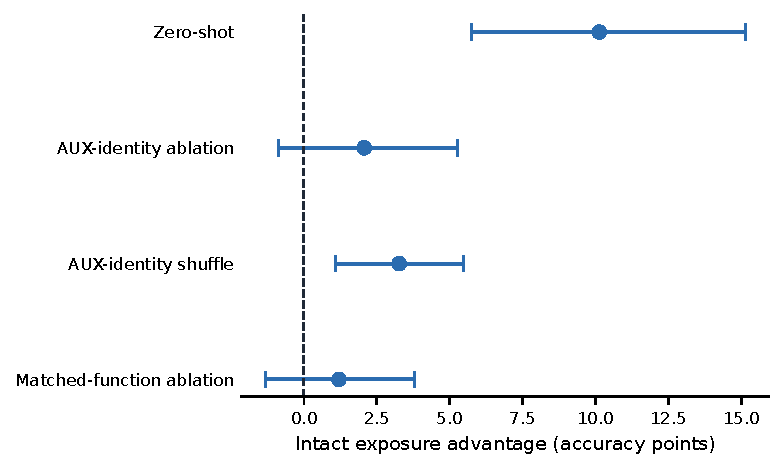
\includegraphics[width=.94\columnwidth]{figures/nonce_effects.pdf}
  \caption{Accuracy advantage of intact nonce-form exposure over each comparison condition. Whiskers are unadjusted 95\% hierarchical paired-bootstrap intervals over three base-model seeds and evaluation items. Holm-adjusted p-values in the text use a different inferential summary, so an interval crossing zero here should not be read as a multiplicity-adjusted test.}
  \label{fig:nonce-effects}
\end{figure}

\section{Discussion}

\paragraph{Total contribution and cue specificity.}
Replacing AUX identities with a shared token reduces performance relative to unchanged training input, but the reduction is not reliably greater than that produced by either matched corpus-damage control on the preregistered metric. Because replacement preserves AUX occurrence and position while changing both form identity and the training distribution, the contrast between the Original and AUX-identity-ablation conditions does not estimate the effect of deleting all auxiliary information. The matched comparisons do not establish an AUX-specific reduction, and their intervals leave room for a small effect.

\paragraph{Evidence for cue integration.}
AUX-only statistics predict verb class above chance, and their diagnosticity is modestly associated with model behavior. POS frames and lexical context are stronger predictors. In the nonce task, AUX-identity shuffling weakens cross-template transfer while preserving the AUX inventory and disrupting its form--context mappings. The matched-function intervention also reduces the continuous preference measure. An alternative explanation is that shuffling lowers local grammatical compatibility, whereas replacement conditions retain position and boundary information; a further possibility is general sensitivity to corpus damage. The present design does not distinguish these mechanisms. It is compatible with a redundant multi-cue account, but does not directly test cue integration.

\paragraph{Scope of the inference.}
The results support a limited claim about text-based learnability: auxiliary patterns can contribute to coarse verb-class expectations within a redundant distributional system. The natural-corpus experiment shows a reliable difference between the Original and AUX-identity-ablation conditions but does not identify an AUX-specific effect; the nonce experiment provides restricted, within-mapping evidence of sensitivity to exposure interventions, while its matched-function-control result again limits a uniqueness claim. They do not show that auxiliaries supply lexical meanings independently or that masked-LM learning reproduces child learning. More generally, the results illustrate the need to compare linguistic ablations with matched-damage and identity interventions when the target cue is correlated with the rest of the training distribution.

\section{Conclusion}

Small masked language models learn coarse verb-class expectations from child-directed text, with auxiliary patterns contributing as part of a broader distributional system. Replacing AUX identities reduces class preference relative to unmodified input, but does not meet the preregistered criterion for an effect beyond either matched-damage control. The baseline and nonce experiments provide compatible evidence that auxiliary patterns are informative, while the stronger lexical and POS-frame baselines and the matched-function-control results do not establish that auxiliaries are uniquely informative. The evidence is compatible with a graded, multi-cue distributional account and illustrates why linguistic ablations require damage-matched controls.

\section*{Limitations}

The task uses a researcher-defined, mixed syntax--semantics ontology rather than a direct measure of complete verb meaning. Its record-level random split does not establish independence at the transcript, speaker, or child level, and the item bootstrap does not separately model clustering by verb, template, transcript, or child. POS tags are assigned automatically. The AUX-identity-ablation token retains the presence and position of the original AUX event, matched controls are not perfectly balanced on every corpus property, and unconstrained AUX-identity shuffling may create locally less compatible sequences. The nonce experiment assigns one form to each class, so nonce identity is not counterbalanced; its three base checkpoints and exposures with highly diagnostic auxiliaries limit generalization. The model is small, English-only, and text-only, and it is a controlled distributional learner rather than a model of child learning.

\section*{Acknowledgements}

I am grateful to Professor Aijun Huang (School of Foreign Languages, Shanghai Jiao Tong University) for guidance throughout the project and detailed feedback on the manuscript. I also thank Dr. Kangzheng Gao for helpful discussions and comments.

\bibliography{references}

\appendix
\section{Training Data Statistics}

This appendix consolidates preprocessing, split, evaluation inventory, and intervention statistics used in the reported experiments. It introduces no additional experiments or outcome measures.

Table~\ref{tab:appendix-data} distinguishes whitespace-delimited tokens in the cleaned corpus from the POS-token units produced after automatic annotation and punctuation segmentation. The deterministic split is performed over model records. Development and test indices are identical across conditions; only the training input is modified.

\begin{center}
  \small
  \setlength{\tabcolsep}{4pt}
  \begin{tabular}{@{}lrr@{}}
    \toprule
    Data stage or split & Records & Units \\
    \midrule
    Cleaned corpus & 904,228 & 6,952,986 \\
    POS-segmented corpus & 904,222 & 8,449,144 \\
    Training split & 723,377 & 6,759,957 \\
    Development split & 90,422 & 844,603 \\
    Test split & 90,423 & 844,584 \\
    \bottomrule
  \end{tabular}
  \captionof{table}{Corpus statistics. ``Records'' denotes cleaned utterances in the first row and model records thereafter. ``Units'' denotes whitespace-delimited tokens in the first row and POS-token units thereafter.}
  \label{tab:appendix-data}
\end{center}

Table~\ref{tab:appendix-pos} reports the complete marginal UPOS percentages over POS-token units in each frozen split.

\begin{center}
  \small
  \setlength{\tabcolsep}{4pt}
  \renewcommand{\arraystretch}{0.94}
  \begin{tabular}{@{}lrrr@{}}
    \toprule
    UPOS & Train (\%) & Dev (\%) & Test (\%) \\
    \midrule
    ADJ   & 3.32  & 3.31  & 3.31 \\
    ADP   & 6.63  & 6.66  & 6.64 \\
    ADV   & 5.37  & 5.37  & 5.34 \\
    AUX   & 11.07 & 11.07 & 11.11 \\
    CCONJ & 2.16  & 2.14  & 2.17 \\
    DET   & 8.54  & 8.57  & 8.51 \\
    INTJ  & 1.82  & 1.80  & 1.85 \\
    NOUN  & 11.32 & 11.29 & 11.28 \\
    NUM   & 0.71  & 0.71  & 0.70 \\
    PART  & 3.93  & 3.93  & 3.94 \\
    PRON  & 16.23 & 16.24 & 16.27 \\
    PROPN & 2.72  & 2.71  & 2.70 \\
    PUNCT & 12.11 & 12.12 & 12.11 \\
    SCONJ & 1.69  & 1.68  & 1.68 \\
    SYM   & 0.01  & 0.01  & 0.01 \\
    VERB  & 12.34 & 12.35 & 12.33 \\
    X     & 0.05  & 0.05  & 0.05 \\
    \bottomrule
  \end{tabular}
  \captionof{table}{Complete UPOS distributions in the frozen splits. Values are percentages and may not sum to exactly 100 because of rounding.}
  \label{tab:appendix-pos}
\end{center}

The two smaller learning-curve samples are nested subsets of the cleaned corpus: the 720k sample contains 93,606 utterances and 719,992 whitespace-delimited tokens, and the 2M sample contains 259,743 utterances and 1,999,991 tokens. The natural-corpus evaluation contains 600 items (120 per class) drawn from 600 distinct records, with 76 target surfaces from 39 lemmas. Its balanced candidate inventory contains 105 surfaces, 21 per class.

The confirmatory training split contains 748,105 AUX events distributed across 543,153 records. Each intervention changes exactly 748,105 positions; Table~\ref{tab:appendix-interventions} shows that matching the number of changed positions does not imply matching the number of affected records. The matched-content and matched-function controls affect 99.4\% and 85.2\%, respectively, as many records as the AUX-targeted intervention. This imbalance is one reason the matched-control contrasts are interpreted conservatively.

\begin{center}
  \small
  \setlength{\tabcolsep}{3.5pt}
  \begin{tabular}{@{}lrr@{}}
    \toprule
    Training condition & Positions & Records \\
    \midrule
    Original & 0 & 0 \\
    AUX-identity ablation & 748,105 & 543,153 \\
    Matched-content ablation & 748,105 & 539,920 \\
    Matched-function ablation & 748,105 & 462,741 \\
    AUX-identity shuffle & 748,105 & 543,153 \\
    \bottomrule
  \end{tabular}
  \captionof{table}{Changed training positions and affected records. Development and test inputs remain unchanged.}
  \label{tab:appendix-interventions}
\end{center}
\vspace{-0.35\baselineskip}

For nonce transfer, each of the five classes has 80 exposure items and 100 evaluation items, for 400 and 500 items in total. Every exposure contains an AUX. Each class uses 15 exposure-frame types, and no exact local $\pm2$ POS frame overlaps between exposure and evaluation. All five nonce forms are absent from the corpus and tokenize into two BPE pieces.

\section{Model Training and Evaluation}

Table~\ref{tab:appendix-training} summarizes the frozen optimization settings. Confirmatory models are trained independently from random initialization. Nonce adaptation starts from the Original-condition checkpoints for seeds 2026--2028 and changes only the exposure input; all nonce evaluation contexts remain intact.

\begin{center}
  \small
  \setlength{\tabcolsep}{3.5pt}
  \begin{tabular}{@{}lcc@{}}
    \toprule
    Setting & Corpus training & Nonce adaptation \\
    \midrule
    Transformer layers & 2 & 2 \\
    Hidden / FF size & 128 / 512 & 128 / 512 \\
    Attention heads & 4 & 4 \\
    Trainable parameters & 946,208 & 946,208 \\
    BPE vocabulary & 4,000 & 4,000 \\
    Epochs & 5 & 8 \\
    Batch size & 16 & 16 \\
    Learning rate & 0.0005 & 0.00005 \\
    Weight decay & 0.01 & 0 \\
    Gradient clipping & 1.0 & -- \\
    MLM probability & 0.15 & target masked \\
    Model seeds & 2026--2030 & 2026--2028 \\
    \bottomrule
  \end{tabular}
  \captionof{table}{Architecture and optimization settings. Nonce runs retain the tokenizer and architecture.}
  \label{tab:appendix-training}
\end{center}

Candidate scoring sums the log probabilities of all BPE pieces for a surface form and divides by the number of pieces. Verb-class accuracy selects the highest-scoring candidate surface and assigns its verb class as the prediction. For \cps{}, scores are first averaged within each class; \cps{} is the mean score of the correct class minus the mean score of the four alternative classes. Confirmatory uncertainty is estimated with 10,000 paired hierarchical-bootstrap samples over seeds and items. Nonce $p$-values are two-sided and Holm-adjusted within the prespecified six-test family.
\end{document}
